\documentclass[12pt,a4paper]{scrartcl}

\usepackage[sc]{mathpazo}
\usepackage[onehalfspacing]{setspace}
\usepackage[T1]{fontenc}
\usepackage[utf8]{inputenc}
\usepackage[ngerman]{babel}
\usepackage{geometry}
\usepackage{amsmath}
\usepackage{amsfonts}
\usepackage{amssymb}
\usepackage{graphicx}
\usepackage{natbib}
\usepackage[hyphens]{url}
\usepackage[printonlyused, withpage]{acronym}
\usepackage{listings}
\usepackage{color}
\usepackage{beramono}
\usepackage{wrapfig}

\geometry{a4paper, portrait, left=2.5cm, right=2.5cm, top=2cm, bottom=2cm}
\parindent0cm

\pagestyle{headings}

\author{Malte Modrow}

\definecolor{lightgray}{rgb}{.9,.9,.9}
\definecolor{darkgray}{rgb}{.4,.4,.4}
\definecolor{purple}{rgb}{0.65, 0.12, 0.82}

\definecolor{gray}{rgb}{0.4,0.4,0.4}
\definecolor{darkblue}{rgb}{0.0,0.0,0.6}
\definecolor{cyan}{rgb}{0.0,0.6,0.6}

\lstdefinelanguage{JavaScript}{
  keywords={typeof, new, true, false, catch, function, return, null, catch, switch, var, if, in, while, do, else, case, break},
  keywordstyle=\color{blue}\bfseries,
  ndkeywords={class, export, boolean, throw, implements, import, this},
  ndkeywordstyle=\color{darkgray}\bfseries,
  identifierstyle=\color{black},
  sensitive=false,
  comment=[l]{//},
  morecomment=[s]{/*}{*/},
  commentstyle=\color{purple}\ttfamily,
  stringstyle=\color{red}\ttfamily,
  morestring=[b]',
  morestring=[b]"
}

\lstdefinelanguage{XML}{
	morestring=[b]",
  	morestring=[s]{>}{<},
  	morecomment=[s]{<?}{?>},
  	stringstyle=\color{black},
  	identifierstyle=\color{darkblue},
  	keywordstyle=\color{cyan},
  	morekeywords={xmlns,version,type}
}

\lstset{
   backgroundcolor=\color{lightgray},
   extendedchars=true,
   basicstyle=\footnotesize\ttfamily,
   columns=flexible,
   frame=single,
   showstringspaces=false,
   showspaces=false,
   numbers=left,
   numberstyle=\footnotesize,
   numbersep=9pt,
   tabsize=4,
   breaklines=true,
   showtabs=false,
   captionpos=b,
   escapechar=',
   inputencoding=utf8,
   belowskip=2em,
   aboveskip=3em,
   literate={Ö}{{\"O}}1{Ä}{{\"A}}1{Ü}{{\"U}}1{ß}{{\ss}}2{ü}{{\"u}}1{ä}{{\"a}}1{ö}{{\"o}}1{©}{{\copyright}}1
}


\begin{document}
\thispagestyle{plain}
\tableofcontents
\thispagestyle{plain}

\newpage
\section{Einleitung}
\label{sec:einleitung}
\newpage
\section{Windows 8}
\label{sec:windows8}
Seit dem 26. Oktober 2012 ist Microsofts aktuellstes Betriebssystem \glqq Windows 8\grqq\ für die breite Öffentlichkeit verfügbar. Dieses unterscheidet sich grundlegend von seinem Vorgänger \glqq Windows 7\grqq. Microsoft verfolgt mit Windows 8 den Ansatz, das gleiche Betriebssystem sowohl für Desktop- als auch für Tablet-Computer\footnote{Tablet-Computer: kleiner, flacher, tragbarer Computer mit einem Touchscreen. Es wird von nun an, der Einfachheit halber die englische Version \glqq Tablet\grqq\ benutzt.} zu verwenden. Es besitzt nach wie vor den bekannten Desktop von Windows 7. Äußerlich sind hier nur kleine Änderungen vorgenommen worden. So besitzt z.B. der Windows Explorer eine neues, kontextsensitives Ribbon-Menü\footnote{Auch bekannt als Menüband oder Multifunktionsleiste.}. Neu ist hingegen das "Modern User Interface" (Modern UI, früher Metro), eine für Touch-Gesten optimierte Oberfläche. Obwohl die neue Oberfläche für Touch-Gesten optimiert ist, kann sie trotzdem auch mit Maus und Tastatur bedient werden. Es können, im Gegensatz zum Desktop, keine herkömmlichen Programme im Modern UI ausgeführt werden. In der Modern UI Oberfläche laufen nur Programme (Apps), die speziell für Windows 8 entwickelt wurden und über den Microsoft Store (siehe Sektion \ref{subsubsec:store} auf Seite \pageref{subsubsec:store}) erhältlich sind. Es soll nun ein etwas detaillierterer Blick auf die neue Oberfläche und dessen Eigenheiten geworfen werden.
\subsection{Neues Bedienkonzept}
\label{subsec:bedienkonzept}
%gesten charms usw

\subsection{Windows 8 als hybrides System}
\label{subsec:hybrides system}
% touch, vorteile, nachteile
Windows 8 kann sowohl auf herkömmlichen Desktop Computern als auch auf Tablet-Computern eingesetzt werden. 
\subsection{Windows RT}
\label{subsec:winRT}
\subsection{Das Ökosystem}
\label{subsec:ökosystem}
\subsubsection{Microsoft Store}
\label{subsubsec:store}
\subsubsection{Windows Phone}
\label{subsubsec:windowsphone}

\newpage
\section{Bildsprache}

\newpage
\section{Konzeption der App}
\label{sec:konzeption}
In diesem Kapitel geht es darum, die Konzeption für eine Windows 8 Nachrichten App darzustellen und zu erläutern. Dabei gilt es darzulegen, warum und mit welchem Hintergrund Entscheidungen zu Gunsten der einen oder der anderen Möglichkeit ausfallen. Dazu müssen zunächst die Ziele der App ausgeführt werden. Anschließend muss sich entschieden werden mit welcher Technologie bzw. Programmiersprache gearbeitet werden soll. Zuletzt wird noch ein detaillierterer Blick auf das Herzstück der App geworfen. Das Navigationskonzept. Hierbei ist eine der wichtigsten Fragen: \glqq Wie kann ich auch bei ggf. großen Datenmengen eine übersichtliche, intuitive Struktur schaffen die sich in das Gesamtkonzept von Windows 8 eingliedert?\grqq  

\subsection{Ziel der App}
\label{subsec:zielderapp}
Das Ziel der zu erstellenden App ist, den Inhalt der ZEIT ONLINE Website auf ansprechende Art und Weise in einer Windows 8 Applikation darzustellen. Das Layout und die Darstellung der Inhalte soll sich an das sogenannte \glqq Look and Feel\grqq\ von Windows 8 anpassen und sich daran orientieren. Der Fokus bei den Inhalten liegt auf den Artikeln selbst und den jeweiligen Aufmacher bzw. Teaser Bildern. Das heißt andere Inhalte wie z.B. Bildergalerien, Infografiken, Blogartikel oder Quizze werden von der App nicht erfasst und nicht dargestellt. Hintergrund ist, die App möglichst einfach zu halten da es in der Fragestellung um die Relation zwischen den Aufmacherbildern und dem dahinter liegenden Artikeltext geht. Die App erhebt in dieser Hinsicht keinen Anspruch darauf, die gesamten redaktionellen Inhalte von \mbox{ZEIT ONLINE} darzustellen, sondern versteht sich eher als explorative Applikation im Sinne der Fragestellung.\\
Der User soll die Möglichkeit haben die standardmäßig vorhandenen Artikeltitel auszublenden um so, wenn gewünscht, einen rein visuellen Eindruck der Artikelbilder zu bekommen. Hierzu soll einen Schalter in der Menüleiste am unteren Bildrand geben. Wenn der User sich im Artikel befindet soll er die Möglichkeit haben die Schriftgröße in gewissen Maß selbst zu bestimmen, da die App eventuell auf Monitoren mit verschieden großen Auflösungen ausgeführt werden wird oder die Sehkraft des Users nicht mehr ausreicht um eine normal große Schrift zu erkennen und zu lesen. So wird in den Artikeln ein gewisses Maß an Barrierefreiheit gewährleistet.\\
Das übergeordnete Ziel der App ist es, eine rudimentäre Nachrichten Applikation für Windows 8 zu erstellen. Gleichzeitig soll eine Umgebung geschaffen werden, die es erlaubt Untersuchungen anzustellen, in wie weit es möglich ist allein durch das Betrachten der Aufmacherbilder auf den Inhalt der jeweiligen Artikel zu schließen (siehe Sektion \ref{subsubsec:nurbildermodus} auf Seite \pageref{subsubsec:nurbildermodus}). Außerdem soll die App dazu dienen, zu erforschen, wie eine Nachrichten Applikation in der Modern UI Oberfläche von Windows 8 erstellt wird und welche design- als auch funktionstechnischen Vorgaben von Microsofts vorhanden sind. Sprich, wie eine App mit Nachrichteninhalten nach Microsofts Sichtweise auszusehen hat. 

\subsection{Nativ vs. Web}
\label{subsec:nativ_vs_web}
Vor dem Entwickeln einer Windows 8 App muss sich entschieden werden mit welcher Technologie bzw. mit welcher Programmiersprache entwickelt werden soll. Die Rede ist hier von einer App die in der Modern UI Oberfläche von Windows 8 läuft und für diese konzipiert ist. Das heißt es handelt sich nicht um eine klassische .NET oder WIN32 Anwendung für Windows. Um eine Modern UI App zu entwickeln, müssen zwei Dinge zwingend vorhanden sein. Zum einen Windows 8 selbst und zum anderen wird die neueste Version von Visual Studio, Visual Studio 11\footnote{Visual Studio 2011 war die aktuellste Version beim Erstellen dieser Arbeit.}, benötigt. Visual Studio steht in der Express Version für Windows 8 kostenlos zur Verfügung. Des weiteren muss sich zwischen der nativen Umsetzung und der Implementierung mit Webtechnologien entschieden werden. Es soll zunächst erläutert werden was die beiden Begriffe bedeuten und in welcher Weise und welchem Zusammenhang sie bei der Entwicklung einer Windows 8 Modern UI App üblicherweise gebraucht werden.

\subsubsection{Native App}
\label{subsubsec:nativ}
Der heutige Begriff \glqq native App\grqq\ unterscheidet sich in einigen Punkten von der früheren oder ursprünglichen Verwendung des Begriffs. Früher sprach man von einer nativen App wenn direkt auf die Ressourcen der  Maschine zugegriffen wurde, wie z.B. Maschinencode der direkt von der CPU ausgeführt wird. Heute wird eine App oftmals schon als nativ deklariert, wenn es sich nicht um eine Webapp handelt. Eine sinnige Definition liegt irgendwo zwischen diesen beiden Varianten. Eine App ist dann nativ, wenn sie Geräte- , Betriebssystem- oder Laufzeitumgebungsabhängig ist. Das heisst, sie ist für ein spezielles Gerät entwickelt und kann nur auf diesem ausgeführt werden. Sie kann dabei alle Geräte- oder Betriebssystemspezifischen Funktionen nutzen, es ist jedoch egal wie nah an der Hardware tatsächlich programmiert wurde \citep{OBrian2013}.\\
In Visual Studio können native Windows 8  Apps u.a. mit den Programmiersprachen C++, C\# oder Visual Basic erstellt werden. Für das Design bzw. das Aussehen der App wird die Markupsprache - \ac{xaml} - verwendet. Es gibt zwei Möglichkeiten wie das \ac{xaml} erstellt werden kann. Es kann entweder von Hand geschrieben werden oder man lässt es sich automatisch generieren. Zum automatischen Generieren lassen sich per Drag \& Drop Elemente wie z.B. Buttons und andere Schaltflächen aus einer Werkzeugpalette direkt auf die \glqq App-Leinwand\grqq\ ziehen, sowie verschieben oder nach Belieben anordnen.
%Listing XAML oder Screenshot 

\subsubsection{Windows 8 App mit Webtechnologien}
\label{subsubsec:webwin8}

\subsection{Navigationskonzept}
\label{subsec:navikonzept}
Damit der User ein für ihn angenehmes und flüssiges Nutzungserlebnis hat, ist es notwendig sich über das Navigationskonzept Gedanken zu machen, gerade wenn es sich um eine App handelt, in der es viele verschiedene Inhaltsbereiche gibt. Der User soll sich möglichst intuitiv durch die Inhalte bewegen können. Außerdem muss dem User auf der Einstiegsebene der ein guter Überblick über die vorhandenen Inhalte gegeben werden, damit er von dort aus zielgerichtet weiter navigieren kann, ohne lange suchen zu müssen. Microsoft nennt in seinen Richtlinien für Windows Store Apps (Modern UI Apps) grundsätzlich zwei Möglichkeiten wie die Navigation umgesetzt werden kann.

\subsubsection{Flaches System}
\label{subsubsec:flachessystem}
Das flache Navigationssystem wird in vielen Windows Store Apps verwendet, häufig in Spielen, Browsern oder in Apps zum Erstellen von Dokumenten. Es zeichnet sich dadurch aus, dass sich die Inhalte auf der gleichen hierachischen Ebene befinden. Dieses System eignet sich wenn ein schneller Wechsel zwischen wenigen Seiten oder Registerkarten möglich sein soll \citep{MicrosoftNavidesign2013}.

\begin{figure}[h]	
	\centering
	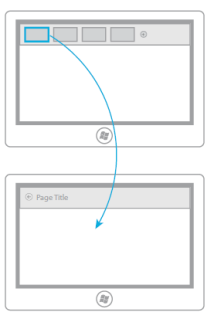
\includegraphics[scale=1]{Bilder/Abbildungen/ms_navigation_flach.png} 
	\caption{Flaches Navigationssystem \protect\citep{MicrosoftNavidesign2013}.}
	\label{fig:naviflach}
\end{figure}

Abbildung \ref{fig:naviflach} zeigt wie das flache Navigationssystem funktioniert. Am oberen Rand befindet sich eine, nicht immer sichtbare Navigationsleiste mit den verschiedenen Registerkarten oder Seiten. Die Leiste wird angezeigt, wenn der User vom unteren oder oberen Bildrand streift (siehe Sektion \ref{subsec:bedienkonzept}). Wenn der User die Seite wechseln möchte geschieht dies  direkt über die Navigationsleiste, d.h. es gibt meist keinen permananten Zurück-Button. Ein flaches Navigationssystem eignet sich nicht unbedingt für eine Nachrichten App wie die, die in dieser Arbeit konzipiert und umgesetzt ist, weil es zu viele Bereiche (Ressorts) gibt, welche sich zudem sehr ähneln. Hier ist es angebracht ein hierarchisches Navigationssystem zu verwenden.    



\subsubsection{Hierarchisches System}
\label{subsubsec:hierachischessystem}
Die meisten Windows Store-App benutzen ein hierarchisches Navigationssystem. Microsoft nennt es Hubnavigationsmuster. Es eignet sich um große Inhaltssammlungen zu ordnen und sie für User benutzerfreundlich auf zu bereiten. Der Schlüssel dazu ist die Unterteilung des Inhalts in verschiedene Detailebenen \citep{MicrosoftNavidesign2013}.

\begin{figure}[h]	
	\centering
	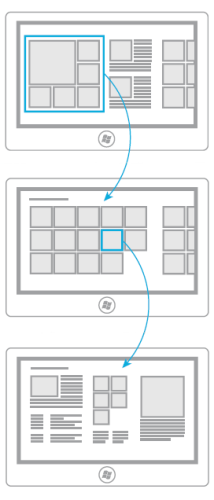
\includegraphics[scale=1]{Bilder/Abbildungen/ms_navigation_hierarchie} 
	\caption{Hierarchisches Navigationssystem \protect\citep{MicrosoftNavidesign2013}.}
	\label{fig:navihierarchisch}
\end{figure}

Das Schema eines hierarchischen Systems ist in Abbildung \ref{fig:navihierarchisch} dargestellt. Der Einstiegspunkt in die App ist die sogenannte \glqq Hubseite\grqq\, hier ganz oben in der Abbildung zu sehen. Auf der Hubebene werden aus den vielen großen Bereichen der App jeweils ein kleiner Teil gesammelt und dargestellt, sodass sich der User vorstellen kann was ihn im jeweiligen Bereich erwartet. Die Anordnung, in welcher der Auszug der Inhalte dargestellt ist muss nicht für jeden Bereich gleich sein. Es kann das Nutzungserlebnis sogar verbessern und vielfältiger machen wenn unterschiedliche Darstellungen (z.B. in Höhe, Breite oder Anzahl der Objekte) für die Bereiche genutzt werden. Die Hubansicht wird horizontal gescrollt, d.h. weiterer Inhalt befindet sich hinter dem rechten Rand und kann entweder durch das Scrollrad der Maus oder auf einem Tablet, durch das swipen nach links in das Sichtfeld des Users gebracht werden.\\
Die mittlere Darstellung in Abbildung \ref{fig:navihierarchisch} zeigt die zweite Detailstufe des hierarchischen Systems. Hier werden alle Elemente eines Bereichs dargestellt. In diesem Fall werden hier alle Artikel aus einem Ressort aufgelistet.\\
Im unteren Bereich der Abbildung ist schließlich die letzte Detailstufe zu sehen. Es handelt sich hierbei um den eigentlichen Inhalt (z.B. einen Artikel). Es ist ebenfalls möglich von der Hubansicht direkt in die Detailansicht eines Elements zu wechseln.  

\begin{figure}[h]	
	\centering
	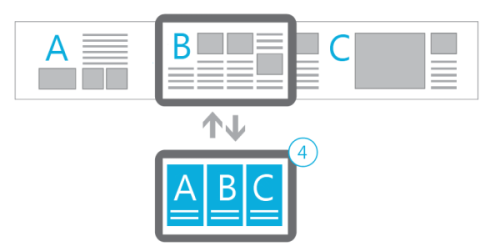
\includegraphics[scale=1]{Bilder/Abbildungen/ms_navigation_hierarchie_semantic_zoom} 
	\caption{Schema des \glqq Semantic Zoom\grqq\ \protect\citep{MicrosoftNavidesign2013}.}
	\label{fig:semanticzoom}
\end{figure}

Befinden sich in der Hubansicht, trotz der Zusammenfassung der Bereiche noch zu viele Bereiche und es dauert zu lange bis zum Ende zu scrollen, kann man noch eine weitere Ebene \glqq davor\grqq\ legen. Das Konzept nennt Microsoft \glqq Semantic Zoom\grqq\ und ist in Abbildung \ref{fig:semanticzoom} schematisch dargestellt. Oben in der Abbildung ist die Hubansicht dargestellt, unten die zusätzliche semantic Zoom Ebene. In der Praxis kann der User auf diese Weise die Inhalte noch weiter vereinfachen und zusammenfassen lassen. Im Fall dieser App soll es einen semantischen Zoom geben, um ein flüssigeres und schnelleres Navigieren z.B. ganz zum Ende der Hubansicht zu ermöglichen, da es über zehn verschiedene Ressorts geben wird. Diese Ansicht soll nur die Namen der verschiedenen Ressorts, sowie ein zufälliges Bild aus dem jeweiligen Ressort zeigen. Um am Desktop-PC (mit Maus) diese Ansicht aufzurufen, muss der User auf ein kleines Minuszeichen am unteren rechten Rand klicken. Am Tablet wird der semantische Zoom mit der \glqq Pinch to Zoom (out)\footnote{Pinch to Zoom erklären}\grqq\  Geste aufgerufen. Klickt der User auf ein Element in dieser zusätzlichen Navigationsebene, wird er direkt zum jeweiligen Ausschnitt in die Hubansicht navigiert. Die semantic Zoom Ansicht kann von überall aus der Hubansicht aufgerufen werden.    


\subsection{Menü und Features}
\label{subsec:menuandproperties}
Da die App einen explorativen Charakter hat wird sich bei den Funktionen und Features auf das nötigste beschränkt. Es soll eine untere App-Leiste geben, in welcher, je nach dem in welcher Ansicht sich der User gerade befindet verschiedene Optionen angezeigt werden. Diese Leiste ist nicht dauerhaft zu sehen und kann, wenn man mit der Maus arbeitet durch einen Rechtsklick aufgerufen werden. Auf einem Tablet geschieht dies durch swipen vom oberen oder unteren Bildschirmrand.\\
In der Startansicht, sowie in der Ressortübersicht soll es am unteren Bildrand die Möglichkeit geben, die Titel aller Elemente aus- bzw. auch wieder einzublenden um so dem User ein rein visuelles Erleben der Artikelbilder zu ermöglichen. In der Artikelansicht soll der User die Möglichkeit haben, die Schriftgröße des Artikels zu vergrößern, zu verkleinern, sowie die Schriftgröße wieder auf ihren Startwert zu setzen. 

\newpage
\section{Umsetzung der App}
\label{sec:umsetzungderapp}

\subsection[Rastervorlage] {Rastervorlage\footnote{Die Namen der verwendeten Dateien in der Rastervorlage wurden mittlerweile von Microsoft geändert.}}
\label{subsec:rastervorlage}
Beim Erstellen einer Windows 8 Modern UI App mit \ac{html} und Javascript bietet Microsoft von Haus aus verschiedene Vorlagen für Visual Studio, welche schon einige Grundfunktionen besitzen und sich so als guter Startpunkt für eine weiterführende App eignen. Die Vorlage die für diese App verwendet wird ist die Raster-App (engl. Grid Application) Vorlage. Sie bietet die Grundarchitektur für ein hierarchisches Navigationssystem wie es in Sektion \ref{subsubsec:hierachischessystem} auf Seite \pageref{subsubsec:hierachischessystem} beschrieben ist.\\
Es wird von Microsoft empfohlen, dass Windows-Store Apps, welche mit \ac{html} und Javascript erstellt werden das single-page Navigationmodell verwenden. Das bedeutet, die Navigation erfolgt nicht über Hyperlinks, sondern die verschiedenen Inhalte werden direkt in die Seite nachgeladen (ähnlich wie ein iframe). Auf diese Weise gibt keine Sichtbare Unterbrechung beim Navigieren (der Bildschirm wird nicht kurz weiß beim Navigieren). Außerdem erzielt man auf diese Weise eine bessere Performance und die App fühlt sich mehr \glqq app-like\grqq\ an. Die Rastervorlage verwendet das single-page Navigationsmodell \citep{MicrosoftSinglePage2013}.\\  

\subsubsection{HTML Dateien}
\label{subsubsec:htmldateien} 
Folgende \ac{html} Dateien sind bereits in der Raster-App Vorlage enthalten:
\begin{description}
	\item[default.html], wird als erstes geladen und enthält das \ac{html} für den Inhalthost (dies ist die Seite in welche die anderen Inhalte im Zuge der single-page Navigation herein geladen werden).
	\item[groupedItems.html], ist der Einstiegspunkt in die App (die Hubansicht).
	\item[groupDetail.html], zeigt alle Elemente eines Bereichs.
	\item[itemDetail.html], Einzelansicht eines Elements.
\end{description}

\subsubsection{Javascript Dateien}
\label{subsubsec:javascriptdateien} 
Folgende Javascript Dateien sind bereits in der Raster-App Vorlage enthalten:
\begin{description}
	\item[default.js], legt fest wie sich die App beim Start verhält.
	\item[groupedItems.js | groupDetail.js | itemDetail.js], sind die Javascript Dateien, welche das Verhalten für die gleichnamigen \ac{html} Dateien festlegen.
	\item[navigator.js], implementiert das hierarchische Navigationssystem, sowie das single-page Navigationmodell.
	\item[data.js], stellt die benötigten Daten für den Rest der App bereit.
\end{description}

\subsubsection{CSS Dateien}
\label{subsubsec:cssdateien} 
\begin{description}
	\item[default.css], enthält Styles für Inhaltshostseite, sowie für die gesamte App.
	\item[groupedItems.css | groupDetail.css | itemDetail.css], 
\end{description}
Diese Vorlage wird nachfolgend angepasst und verändert, sodass sie die konzeptionierten Anforderungen erfüllt.

\subsection{Datenanbindung}
\label{subsec:datenanbindung}

\subsubsection{ZEIT ONLINE Datenbestand}
\label{subsubsec:zondatenbestand}
Es soll zunächst geklärt werden wie sich der Inhalt der ZEIT ONLINE Website darstellt und wie er generiert wird. Die redaktionellen Inhalte werden fast ausschließlich über ein hauseigenes \ac{cms} erstellt und gepflegt. Das \ac{cms} generiert aus den Inhalten eine \ac{xml}-Struktur. Aus dem \ac{xml} wiederum wird anschließend mit Hilfe von \ac{xslt} in einer zweistufigen Transformation das fertige \ac{html} erstellt. Dies ist ein grober Überblick wie sich die Webseite von ZEIT ONLINE zusammensetzt.\\
Für die Windows 8 App wird direkt das \ac{xml} verwendet, welches vom \ac{cms} generiert wird. Für die App werden zwei verschiedene Seitentypen der Webseite benötigt um die gewünschten Informationen darzustellen. Zum einen die verschiedenen \glqq Centerpages\grqq\ und zum anderen die Artikelansicht. Centerpages sind die Hauptseiten der jeweiligen Ressorts (z.B. die Hauptseite des Politikressorts), sowie die Startseite mit den wichtigsten und aktuellsten Meldungen. Auf den Centerpages befinden sich die Teaserelemente für die verschiedenen Artikel. Die Teaserelemente bestehen meist aus einem Bild und einem kurzen, prägnanten Text, welcher kurz erläutert worum es in dem dahinter liegenden Artikel geht.\\

\begin{minipage}{\linewidth}
\begin{lstlisting}[language= XML,caption=Das XML eines Teaserelements, label={lst:knopfxml}]
<block href="http://xml.zeit.de/digital/internet/2013-08/fablab-open-hardware" year="2013" issue="34" ressort="Digital" author="Tilman Baumgärtel" contenttype="article" publication-date="" expires="" date-last-modified="2013-08-14T12:58:40+00:00" date-first-released="2013-08-14T09:57:43.627551+00:00" date-last-published="2013-08-14T12:59:39.691370+00:00" last-semantic-change="2013-08-14T09:56:40.185797+00:00">
	<supertitle>Open Hardware</supertitle>
	<title>Fab Labs, die Maschinen-Bibliotheken</title>
	<text>
		3-D-Drucker, CNC-Fräsen oder Lasercutter - mit solchen Maschinen sollen Bastler in Fab Labs experimentieren. Immer mehr solcher Werkstätten entstehen nun in aller Welt.
	</text>
	<description>
		3-D-Drucker, CNC-Fräsen oder Lasercutter - mit solchen Maschinen sollen Bastler in Fab Labs experimentieren. Immer mehr solcher Werkstätten entstehen nun in aller Welt.
	</description>
	<byline/>
	<image alt="MakerBot Replicator 2" align="left" title="MakerBot Replicator 2" base-id="http://xml.zeit.de/digital/internet/2013-08/makerbot-cebit-hannover/" type="jpg" publication-date="" expires="">
		<bu>
			Ein MakerBot Replicator 2 auf der diesjährigen Cebit in Hannover
		</bu>
		<copyright>© REUTERS/Fabrizio Bensch</copyright>
	</image>
</block>
\end{lstlisting}


\end{minipage}

Das \ac{xml} von einem Teaserelement ist in Listing \ref{lst:knopfxml} dargestellt. Es werden jedoch nicht alle Informationen aus dem \ac{xml} verwendet. Die verwendeten Informationen sind das \glqq date-first-released\grqq\ (Zeile 1), der \glqq title\grqq\ (Zeile 3), sowie die \glqq description\grqq\ (Zeile 7) und das \glqq image\grqq\ (Zeile 11). Das \ac{xml} für die Artikelansicht ist ähnlich aufgebaut, nur ist hier zusätzlich noch der Artikeltext (Inhalt) in Form von Paragraphen-Tags (<p>) enthalten. Dies ist ein konkreter Einblick wie die rohen Daten aussehen, welche für die App verwendet werden. Wie die Daten im Detail verarbeitet werden wird in der nächsten Sektion erläutert.

\subsubsection{Daten verfügbar machen}
\label{subsubsec:datenverfügbarmachen}
Die Daten, die in der App dargestellt werden sollen, werden grundsätzlich in zwei Schritten geladen. Wenn die App startet werden zunächst alle benötigten Daten außer den eigentlichen Artikeln geladen. Der Artikelinhalt wird erst geladen, wenn der User ihn lesen will. Dies spart Zeit beim starten der App und der User hat somit ein flüssigeres App-Erlebnis. Der erste Schritt beim Daten Einlesen und Verarbeiten geschieht in der \glqq data.js\grqq\ Datei. Es werden alle Teaser Elemente aller Ressorts letztendlich in einer \glqq WinJS.Binding.List()\grqq\ gespeichert und für den weiteren Gebrauch verfügbar gemacht. Die \ac{winjs} ist eine Javascript Bibliothek für Windows-Store Apps, die mit Javascript erstellt werden. Sie enthält nützliche Funktionen z.B. für UI Steuerelemente oder sie hilft beim \ac{xhr}. Die Binding.List ist ebenfalls ein Teil dieser Bibliothek. Sie stellt Logik für die Datengruppierung bereit, genau in der Art und Weise wie es für diese App sinnvoll ist. Falls mit dynamischen Daten gearbeitet wird stellt sie z.B. Funktionen für die automatische Aktualisierung der Daten bereit.In Listing \ref{lst:bindinglst} ist die Initialisierung einer WinJS.Binding.List dargestellt.

\begin{minipage}{\linewidth}
\begin{lstlisting}[language= Javascript,caption=Initialisierung der Binding-List., label={lst:bindinglst}]
var teaserElements = new WinJS.Binding.List();
\end{lstlisting}
\end{minipage}

Die Grundinformationen zu den einzelnen Ressorts, wie der Name und die URL, werden zunächst als normales Javascript Array festgelegt. Einen Beispieleintrag aus dem Array zeigt Listing \ref{lst:ressortsarray}.

\begin{minipage}{\linewidth}
\begin{lstlisting}[language= Javascript,caption=Auszug aus dem Ressorts Array., label={lst:ressortsarray}]
ressorts = [
	{
	    key: "ressort01", url: 'http://xml.zeit.de/index',
	    title: 'Top Stories', subtitle: 'subtitle', updated: 'tbd',
	    backgroundImage: 'tbd', articleLink: "tdb",
	    acquireSyndication: acquireSyndication, dataPromise: null
    }
]
\end{lstlisting}
\end{minipage}

Anschließend wird eine weitere Funktion von \ac{winjs} verwendet, die WinJS.Promises. Mit Promises kann mit asynchronen Prozessen und Datenquellen umgegangen werden. Hier werden für alle Ressorts \ac{xhr}s gestartet, an die im Ressorts-Array angegebene URLs. Alle \ac{xhr}s werden ebenfalls in einem Array gespeichert und erst wenn alle Promises vorhanden sind (alle URL waren erreichbar), wird die Datenverarbeitung fortgesetzt. \\
Mit den vorhandenen und validen \ac{xhr} Responses können anschließend alle Teaserelemente in einer Schleife durchlaufen, das \ac{xml} geparst und so die nötigen Informationen für die App verfügbar gemacht werden. Listing \ref{lst:xmlparsing} zeigt wie der Titel (Zeile 10), der Teasertext (Zeile 13) und der Bildpfad (Zeilen 15-22) aus dem \ac{xml} gewonnen werden. Am Ende der Funktion werden die Daten in die in Listing \ref{lst:bindinglst} erstellte WinJS.Binding.List geschrieben (Zeilen 24-28). Die dargestellte Funktion ist nicht vollständig und wurde aus Übersichts- und Relevanzgesichtspunkten verkürzt dargestellt.

\begin{minipage}{\linewidth}
\begin{lstlisting}[language= Javascript,caption=Parsen und Speichern der Daten., label={lst:xmlparsing}]
function getItemsFromXml(ressortXML, teaserElements, ressort) {
    var teasers = ressortXML.querySelectorAll("region[area='lead'] container > block:first-child");
    // Process each ressort teaser.
    for (var teaserIndex = 0; teaserIndex < teasers.length; teaserIndex++) {
        var teaser = teasers[teaserIndex];

       //only articles with an image are alllowed
        if (teaser.getAttribute("contenttype") == "article" && teaser.querySelector("image") !== null) {
            // Get the title
            var teaserTitle = teaser.querySelector("title").textContent;
        
            // Process the content so that it displays nicely.
            var staticContent = toStaticHTML(teaser.querySelector("description").textContent);

            //Get and build the image path
            var teaserImageEl = teaser.querySelector("image");
            var imageBasePath = teaserImageEl.getAttribute("base-id");
            var splitImagePath = imageBasePath.split('/');
            var imageNameSmall = splitImagePath[splitImagePath.length - 2] + "-220x124.jpg";
            var imageNameBig = splitImagePath[splitImagePath.length - 2] + "-540x304.jpg";
            var imagePathSmall = imageBasePath + imageNameSmall;
            var imagePathBig = imageBasePath + imageNameBig;
            
            // Store the teaser element info we care about in the array.
            teaserElements.push({
                group: ressort, key: ressort.title, title: teaserTitle,
                backgroundImage: imagePathBig, teaserText: staticContent
            });
        }
    }
}
\end{lstlisting}   
\end{minipage}

Sobald die Daten in der WinJS.Binding.List gespeichert sind können sie vom Rest der App weiterverwendet und grafisch aufbereitet werden. Es wurden bisher noch keine Artikelinhalte geladen, dies geschieht erst wenn der User auf einen Artikel klickt.

\subsection{Darstellung der Daten}
\label{subsec:darstellungderdaten}

\subsubsection{Die Hubansicht}
\label{subsubsec:hubansicht}
Wenn die App startet befindet sich der User in der Hubansicht. Hier werden ihm für alle Hauptressorts die ersten sechs Artikel angezeigt, in der Reihenfolge wie sie auch auf der Webseite zu finden sind (siehe Abbildung \ref{fig:hubressortübersicht}).\\
Zu der Hubansicht gehören eine \ac{html} Datei, in welcher das Markup festgelegt ist, eine CSS Datei, die das Layout der Seite bestimmt und eine Javascript Datei, in welcher das Verhalten (die Logik) der Hubseite programmiert wird. 

\begin{figure}[h]
	\centering
	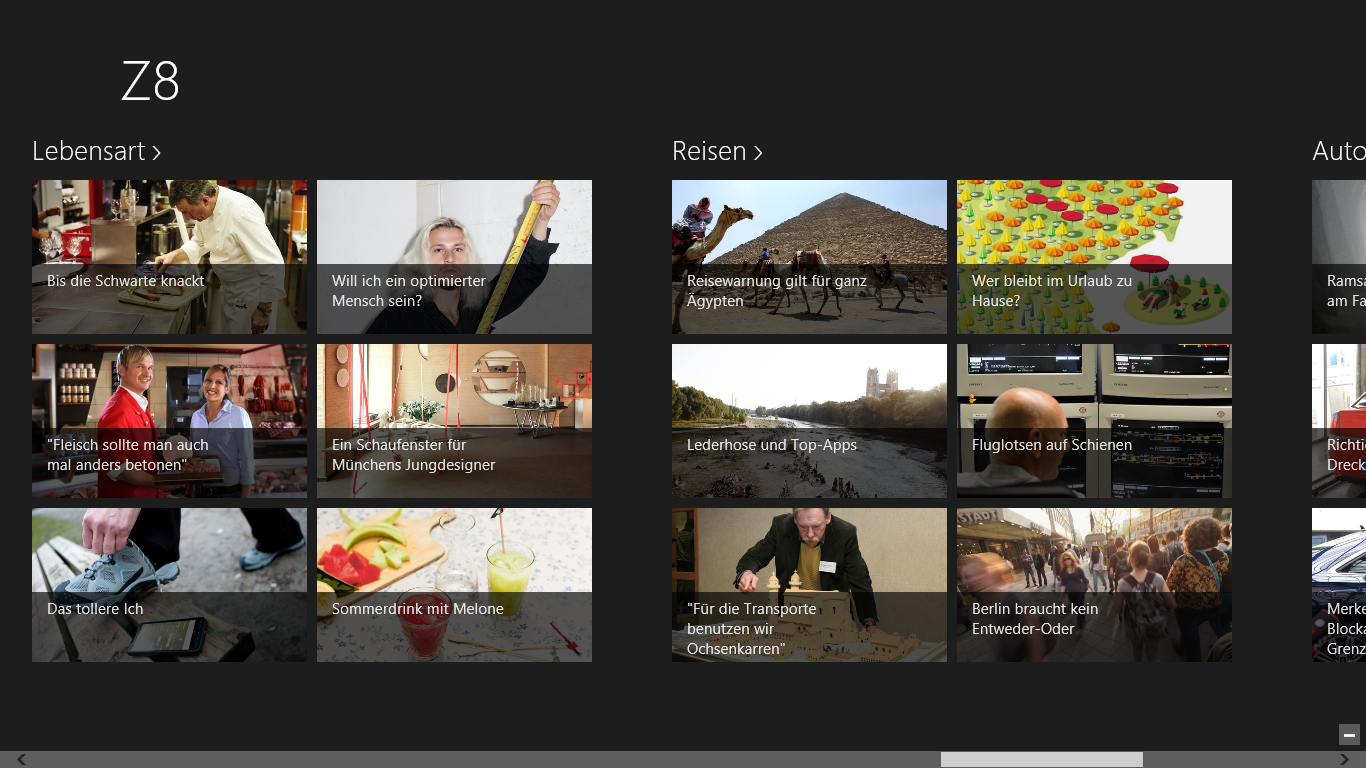
\includegraphics[width=\textwidth]{Bilder/Screenshots/app/reise_aegypten_2gmit.png} 
	\caption{Die Hubansicht.}
	\label{fig:hubressortübersicht}
\end{figure}

Um die Daten aus der \textit{WinJS.Binding.List} auf der Hubseite anzeigen zu können, sind einige Schritte notwendig. Zunächst soll der Aufbau der \ac{html} Datei erläutert werden. Listing \ref{lst:hubmarkup} zeigt einen Ausschnitt aus der \textit{groupedItems.html} Datei. Im oberen Teil befindet sich ein Template mit der Klasse \textit{itemtemplate}, welches auf jedes einzelne Element der Hubansicht angewandt wird. Das besondere an diesem Template ist, dass es ein \textit{data-win-control} Attribut mit dem Wert \glqq WinJS.Binding.Template\grqq\ besitzt. Dies bedeutet, es akzeptiert Daten aus einer \textit{WinJS.Binding.List}, wie sie in der Rohdatenverarbeitung genutzt wurde. Im unteren Teil ab Zeile 10 ist der Container für den eigentlichen Inhalt. Dieses Objekt besitzt ein \textit{data-win-control} Attribut mit dem Wert \glqq WinJS.ListView\grqq\ . Eine \textit{WinJS.LisView} stellt Elemente in anpassbaren Listen oder Rastern dar. 

\begin{minipage}{\linewidth}
\begin{lstlisting}[language= XML,caption=Die wichtigsten Markupelemente der Hubansicht., label={lst:hubmarkup}]
<div class="itemtemplate" data-win-control="WinJS.Binding.Template">
    <div class="item">
        <img class="item-image" src="#" data-win-bind="src: backgroundImage; alt: title" />
        <div class="item-overlay">
            <h4 class="item-title" data-win-bind="textContent: title"></h4>
        </div>
    </div>
</div>

<section aria-label="Main content" role="main">
    <div class="groupeditemslist win-selectionstylefilled" aria-label="List of groups" data-win-control="WinJS.UI.ListView" data-win-options="{selectionMode: 'none'}"></div>
</section>
\end{lstlisting}   
\end{minipage}

Der Rest passiert in der \textit{groupedItems.js} Datei. Die \textit{groupedItems.js} besitzt eine \textit{ready()} Methode. Diese wird jedesmal aufgerufen, wenn der User zur Hubansicht wechselt oder die Hubansicht wiederhergestellt wird. Um die Daten in die \textit{WinJs.ListView} zu bekommen wird als erstes die \textit{WinJS.ListView} in einer Variable gespeichert und anschließend das gewünschte Template bei der ListView registriert (siehe Listing \ref{lst:getitemtemplate}). 

\begin{minipage}{\linewidth}
\begin{lstlisting}[language= Javascript,caption=Template bei der Listview registrieren., label={lst:getitemtemplate}]
var listView = element.querySelector(".groupeditemslist").winControl;
listView.itemTemplate = element.querySelector(".itemtemplate");
\end{lstlisting}   
\end{minipage}

Anschließend wird die \textit{initializeLayout} Funktion aufgerufen. Hier wird am Anfang eine entscheidende Operation ausgeführt. In der \textit{WinJS.Binding.List} sind bisher alle Teaserelemente aus allen Ressorts enthalten, für die Hubansicht sind aber nur sechs Elemente pro Ressort gewünscht. Deswegen wird eine Funktion \textit{getClippedList()} in der \textit{data.js} Datei aufgerufen, welche die ersten sechs Elemente jedes Ressorts zurück liefert. Damit die Elemente wie gewünscht angezeigt werden können, muss noch die \textit{dataSource} der \textit{WinJS.ListView} gesetzt werden, ebenso wie das Raster-Layout (siehe Listing \ref{lst:setdatasource}). Nach diesem Schritt werden die ersten sechs Elemente jedes Ressorts wie in Abbildung \ref{fig:hubressortübersicht} angezeigt.

\begin{minipage}{\linewidth}
\begin{lstlisting}[language= Javascript,caption=Setzen der Datenquelle und des Layouts., label={lst:setdatasource}]
listView.itemDataSource = groupedItemsHub.dataSource;
listView.layout = new ui.GridLayout({ groupHeaderPosition: "top" });
\end{lstlisting}   
\end{minipage}

\subsubsection{Die Ressortansicht}
\label{subsubsec:ressortansicht}
Die Ressortansicht, die zweite Detailstufe zeigt alle Elemente eines Ressorts (siehe Abbildung \ref{fig:einzelressortübersicht}). Der User gelangt hierhin wenn er in der Hubansicht auf den Ressortnamen im Headerbereich klickt. 

\begin{figure}[h]
	\centering
	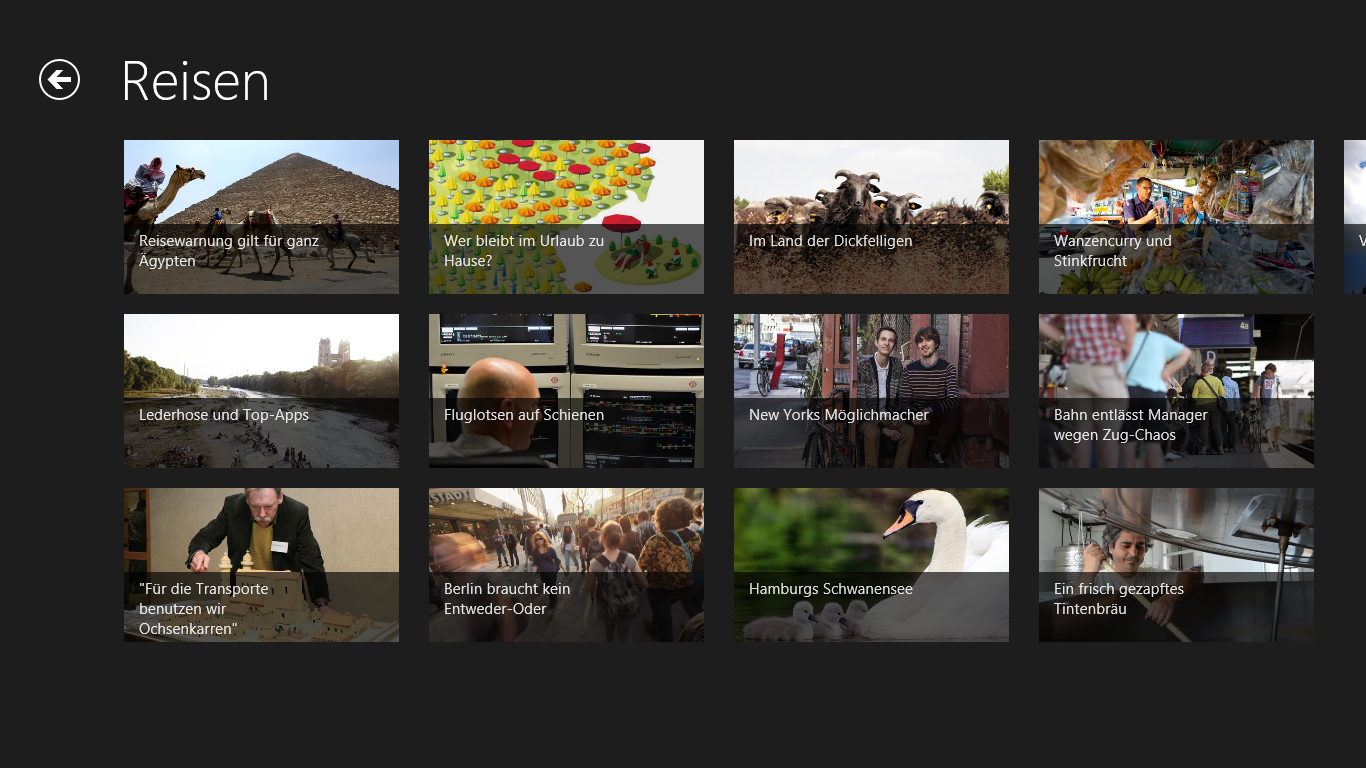
\includegraphics[width=\textwidth]{Bilder/Screenshots/app/reise_aegypten_3gdmit.png} 
	\caption{Die Einzelressortübersicht (hier das Reisen Ressort).}
	\label{fig:einzelressortübersicht}
\end{figure}

Die Programmlogik funktioniert analog zur Hubansicht. Es werden die gleichen Mechanismen zur Darstellung des Raster-Musters benutzt. Auch die zu dieser Ansicht gehörende \ac{html} und Javascript Dateien ähneln denen von der Hubansicht sehr. Ein wesentlicher Unterschied ist, dass im Gegensatz zu Hubansicht nicht die Funktion \textit{getClippedList()}, sondern stattdessen die Funktion \textit{getItemsFromGroup()} aufgerufen wird. Sie gibt alle Elemente der übergebenen Gruppe zurück. Diese können nun mit einem \textit{itemTemplate} und einer \textit{WinJS.ListView} dargestellt werden. 

\subsubsection{Die Artikelansicht}
\label{subsubsec:artikelansicht}
Die Artikelansicht ist die letzte Detailstufe. Sie zeigt den eigentlichen Artikelinhalt (siehe Abbildung \ref{fig:artikelansicht}). Dargestellt wird das Ressort, der Titel, der Teasertext, das Aufmacherbild in groß, die Bildunterschrift, das Copyright für das Bild, der Artikeltext, die Quelle des Artikels (z.B. ZEIT ONLINE oder dpa), der Autor sowie das Erstellungsdatum. Die Artikeldarstellung funktioniert etwas anders als die Hub- und der Ressortdarstellung. Es wird kein Template verwendet, stattdessen wird das \ac{html} mit Hilfe von Javascript befüllt. In der \textit{ready()} Funktion der \textit{itemDetail.js} Datei werden zunächst die bereits vorhandenen Information in das \ac{html} eingefügt.

\begin{figure}[h]
	\centering
	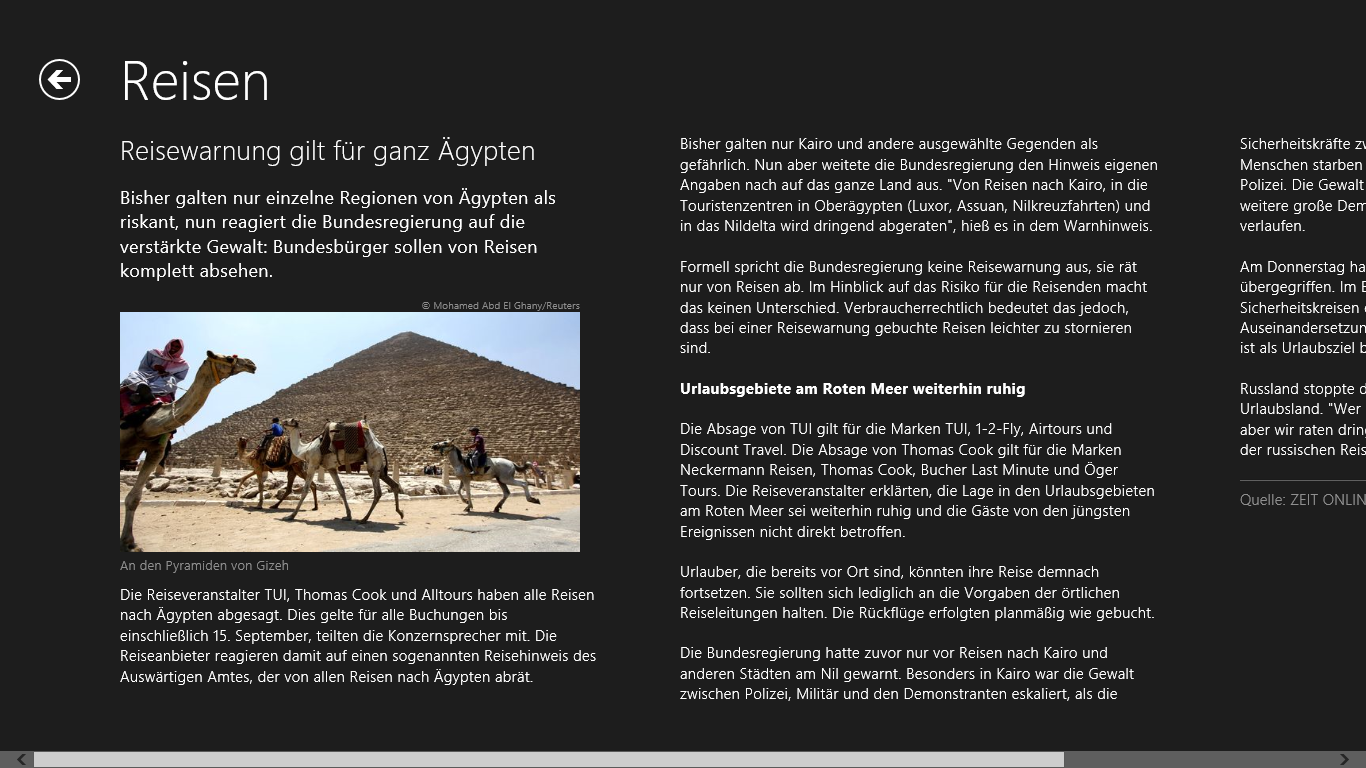
\includegraphics[width=\textwidth]{Bilder/Screenshots/app/reise_aegypten_4d.png} 
	\caption{Die Artikelansicht.}
	\label{fig:artikelansicht}
\end{figure}

Listing \ref{lst:artikelinfos} zeigt das Einfügen von Titel, Teasertext und  dem Bild. Anschließend fehlt noch der Artikeltext, die Quelle und der Autor. Um diese Daten zu bekommen und zu speichern ist ein weiterer \ac{xhr} nötig. Der \ac{xhr} wird mit der Artikel-URL aufgerufen, welche in jedem Teaserelement gespeichert ist. Auf diese Weise bekommt man das \ac{xml} der Artikel, wie es auch von der Webseite verwendet wird. Beim Parsen des Artikel-\ac{xml}s müssen drei Dinge besonders beachtet werden.

\begin{minipage}{\linewidth}
\begin{lstlisting}[language= Javascript,caption=Das Einfügen von Titel sowie Teasertext und Bild., label={lst:artikelinfos}]
element.querySelector("article .item-title").textContent = item.title;
element.querySelector("article .item-subtitle").innerHTML= item.teaserText;
element.querySelector("article .item-image").src = item.backgroundImage;
\end{lstlisting}   
\end{minipage}

Die Absätze des Artikels liegen in Paragraphen-Tags (<p></p>) vor. Es kann vorkommen, das außer dem reinen Text, zusätzlich noch Infoboxen im Artikel vorhanden sind. Ebenso ist es möglich, dass Nachrichten vom Mikroblogging Dienst Twitter eingebunden werden. Diese Abschnitte arbeiten ebenfalls mit Paragraphen-Tags. Da Infoboxen und Twitternachrichten sich inhaltlich nicht direkt in den Artikeltext eingliedern, müssen diese Abschnitte vorher herausgefiltert werden. Des weiteren sind in den meisten Artikeln auf der ZEIT ONLINE Webseite Hyperlinks, entweder auf andere Artikel oder auch andere Webseiten, vorhanden. Diese sind genau wie Infoboxen und Twitternachrichten unerwünscht, da sie, wenn sie vom User aufgerufen werden, in einer andere App (Internet Explorer) geöffnet werden würden. Dies unterbricht und stört das App-Erlebnis. Es muss dementsprechend darauf geachtet werden, dass nur der reine Artikeltext als Artikel gespeichert wird. Listing \ref{lst:artikelabsätze} verdeutlicht wie dies passiert. In Zeile 3 werden die Infoboxen und die Twitternachrichten herausgefiltert und in den Zeilen 8-13 werden die \textit{<a></a>} Tags mit Hilfe regulärer Ausdrücke gelöscht. Sobald der Artikel komplett geladen ist, wird er analog zu Listing \ref{lst:artikelinfos} in das \ac{html} Markup eingefügt.

\begin{minipage}{\linewidth}
\begin{lstlisting}[language= Javascript,caption=Vermeidung von Infoboxen \, Twitternachrichten und Hyperlinks in den Artikeln., label={lst:artikelabsätze}]
for (var n = 0; n < paragraphs.length; n++) {
    //exclude info box and tweets paragraphs
    if (paragraphs[n].parentNode.parentNode.parentNode.parentNode.nodeName != "infobox" && paragraphs[n].parentNode.getAttribute("class") != "twitter-tweet"){
        var xmlText = new XMLSerializer().serializeToString(paragraphs[n]);
        if (paragraphs[n].querySelector("a") != null) {
            var numberOfLinks = paragraphs[n].querySelectorAll("a").length;
            //remove hyperlinks
            for (var i = 0; i < numberOfLinks; i++) {
                var rx = new RegExp("<a[^<>]+>", "i");
                xmlText = xmlText.replace(rx, "");
                rx = new RegExp("</a>", "i");
                xmlText = xmlText.replace(rx, "");
            }
        }
        textContent = textContent + xmlText;
    }
}
\end{lstlisting}   
\end{minipage}

\subsection{Features}
\label{subsec:features}

\subsubsection{Artikeltitel ausblenden}
\label{subsubsec:artikeltitelausblenden}
Ein Hauptfeature der App ist es, dass in der Hubansicht und in der Ressortansicht die Artikeltitel ausgeblendet werden können und der User so nur noch eine Bilderwand vor sich hat. So kann er die Nachrichtenlage rein visuell erleben und erst wenn er auf einen Artikel klickt bekommt er im Artikel den Titel und Artikelinhalt zu sehen. Diese Funktion wird über eine Menüleiste am unteren Bildrand implementiert (siehe Abbildung \ref{fig:menubartitletoggle}). Um eine solche Menüleiste zu erzeugen genügt ein \textit{<div>} Container in der \textit{default.html} Datei mit einem \textit{data-win-control} Attribut, das den Wert \glqq WinJS.UI.AppBar\grqq\ bekommt. In diesem Element können anschließend \textit{<button>} Elemente angelegt werden. Diese sind später die sichtbaren Schaltflächen wenn die Menüleiste aufgerufen wird.

\begin{figure}[h]
	\centering
	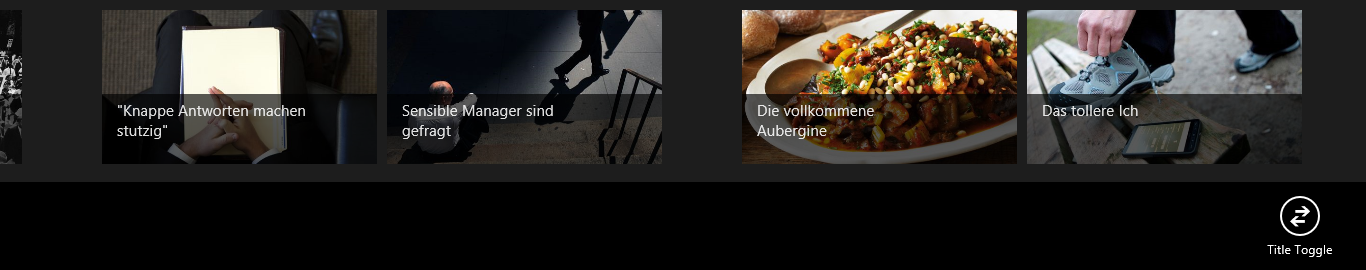
\includegraphics[width=\textwidth]{Bilder/Screenshots/app/title_toggle_menu_bar.png} 
	\caption{Untere Menüleiste mit der Funktion zum Artikeltitel ausschalten.}
	\label{fig:menubartitletoggle}
\end{figure}

In der Initialisierungsphase der App wird in der \textit{default.js} Datei der Click-Handler für den Button registriert. D.h. hier wird die Funktion angegeben, welche aufgerufen werden soll wenn der Button geklickt wird. In diesem Fall wird die Funktion \textit{titleToggle()} in der \textit{globals.js} Datei aufgerufen. In der \textit{globals.js} Datei befinden sich Variablen und Funktionen, die von mehreren Ansichten benutzt werden und deswegen global verfügbar sein sollen. Die \textit{titleToggle()} Funktion ist schließlich verantwortlich für das ausblenden der Artikeltitel.\\
Die Funktion sammelt dazu alle Elemente mit der Klasse \textit{item-overlay} in einem Array und setzt anschließend für alle gefundenen Elemente die CSS Eigenschft \textit{display} auf \glqq none\grqq\ . Das Resultat ist in Abbildung \ref{fig:ressortohnetitel} zu sehen.

\begin{figure}[h]
	\centering
	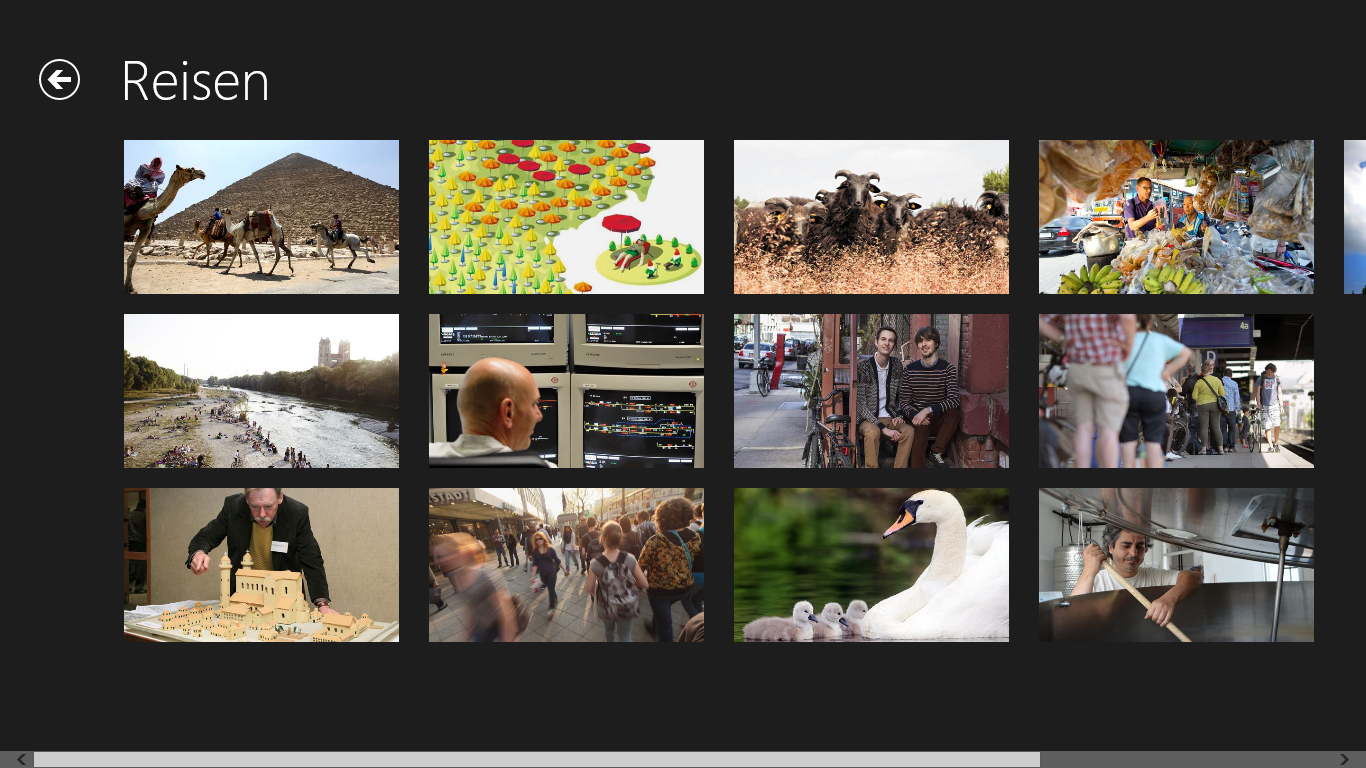
\includegraphics[width=\textwidth]{Bilder/Screenshots/app/reise_aegypten_3gdohne.png} 
	\caption{Das Reisen Ressort ohne Artikeltitel.}
	\label{fig:ressortohnetitel}
\end{figure}

\subsubsection{Schriftgröße verändern}
\label{subsubsec:schriftgroesseveraendern}
In der Artikelansicht hat der User die Möglichkeit, die Schriftgröße anzupassen. Es sind jeweils zwei Stufen größer, als auch zwei Stufen kleiner als die normale Größe möglich. Der  Ansatz ist grundsätzlich genau so wie bei der \glqq Titel-ausblenden\grqq\ Funktionalität. Zunächst wird ein Button in der unteren Menüleiste angelegt. Es wäre auch möglich zwei Buttons zu erstellen, einen für größer und einen für kleiner. Um die Entwicklungsmöglichkeiten jedoch weiter aus zu reizen gibt es in der App nur einen Button in der Menüleiste. Wird dieser geklickt erscheint noch ein weiteres Menü, ein sogenanntes \textit{Flyout-Menü}. In diesem sind schließlich die Schaltflächen für \glqq Schrift größer\grqq\ , \glqq Schrift kleiner\grqq\ und für \glqq Schriftgröße zurücksetzen\grqq\ . Ist die Schriftgröße z.B. auf der größten Stufe eingestellt, wird im Menü, der größer Button nicht mehr dargestellt. Abbildung \ref{fig:fontsizemenü} zeigt die verschiedenen Stati, die das Schriftgrößenmenü haben kann.

\begin{figure}[h]
	\centering
	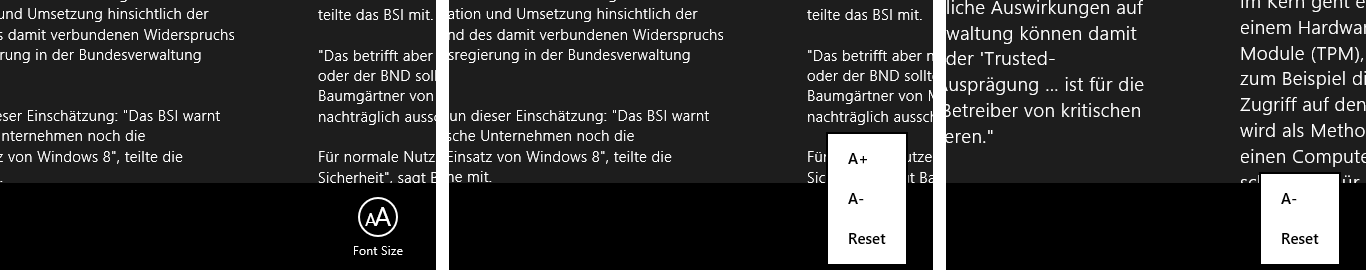
\includegraphics[width=\textwidth]{Bilder/Screenshots/app/font_size_menu_kompakt.png} 
	\caption{links: Schriftgröße Button im unteren Menü | mitte: Das Flyout-Menü mit allen Schaltflächen. | rechts: Das Flyout-Menü beim Aufruf wenn schon die größte Größe eingestellt ist.}
	\label{fig:fontsizemenü}
\end{figure} 

\subsubsection{Semantic Zoom}
\label{subsubsec:semanticzoom}

\subsection{Entwicklungschronologie}
\label{subsec:entwicklungschronologie}


\newpage
\section{Evaluierung} 
\label{sec:evaluierung}

\subsection{Fokusgruppe}
\label{subsec:fokusgruppe}

\subsection{Interview}
\label{subsec:interview}

\subsubsection{Intuitivität der App} 
\label{subsubsec:intuitivitätderapp}

\subsubsection{Der nur Bilder Modus}
\label{subsubsec:nurbildermodus}

\subsection{Ergebnis}
\label{subsec:ergebnis}

\newpage
\section{Fazit}
\label{sec:fazit}

\newpage
\section*{Abkürzungsverzeichnis}
\label{sec:abkürzungen}
\begin{acronym}[SEPSEP]
	\acro{xaml}[XAML]{Extensible Application Markup Language}
	\acro{cms} [CMS]{Content Management System}
	\acro{xml} [XML]{Extensible Markup Language}
	\acro{xslt}[XSLT]{Extensible Stylesheet Language Transformations}
	\acro{html}[HTML]{Hypertext Markup Language}
	\acro{xhr}[XHR]{XMLHttpRequest}
	\acro{winjs}[WinJS] {Windows Library for JavaScript}
\end{acronym}

\newpage
\begin{singlespace}
	\bibliographystyle{natdin}
	\bibliography{ba_literatur}
\end{singlespace}

\newpage
\listoffigures

\newpage
\lstlistoflistings


\end{document}